\documentclass[runningheads]{llncs}
\usepackage{graphicx}
\usepackage{booktabs}
\usepackage{amsmath}
\usepackage{url}
\usepackage{microtype}

\renewcommand{\topfraction}{0.95}
\renewcommand{\bottomfraction}{0.95}
\renewcommand{\textfraction}{0.05}
\renewcommand{\floatpagefraction}{0.90}
\setlength{\abovecaptionskip}{4pt}
\setlength{\belowcaptionskip}{2pt}
\setlength{\textfloatsep}{8pt plus 2pt minus 2pt}
\setlength{\floatsep}{8pt plus 2pt minus 2pt}

\begin{document}

\title{VLM3D Classification: Multi-Label Chest CT Anomaly Detection}
\titlerunning{VLM3D: Multi-Label Chest CT Anomaly Detection}

\author{Sourabh Kumawat}
\authorrunning{S. Kumawat}

\institute{University College Dublin, Dublin, Ireland \\
\email{sourabh.kumawat@ucdconnect.ie}}

\maketitle

\begin{abstract}
Automated multi-label anomaly detection from volumetric computed tomography (CT) requires balancing computational tractability, fine-grained lesion sensitivity, and global anatomical context. We present a multi-backbone classification pipeline for the VLM3D Challenge Task~1 (18 thoracic pathologies on the CT-RATE dataset). The proposed system integrates dynamic percentile Hounsfield Unit (HU) windowing, an architectural progression spanning 3D ResNet, DenseNet201, and a SuPreM-pretrained SwinViT-3D, Asymmetric Loss (ASL) with weak-class parameter tuning, 8-fold test-time augmentation (TTA), and Nelder-Mead simplex ensembling with per-class decision threshold calibration. The final ensemble achieves a macro AUROC of 0.8025 and macro F1 of 0.5212 across 3,039 held-out validation scans, substantially outperforming the official CT-Net (0.762 AUROC) and CT-CLIP (0.735 AUROC) baselines. Diagnostic ablations demonstrate that resolving an initial static HU clipping failure provided the largest single gain (+0.18 AUROC), while domain-specific supervised pre-training and calibrated ensembling yielded the remaining state-of-the-art margins.
\keywords{3D CT classification \and Multi-label learning \and Swin Transformer \and Asymmetric Loss \and Ensembling \and CT-RATE}
\end{abstract}

\section{Introduction}
Computed tomography (CT) of the thorax is the diagnostic gold standard for evaluating pulmonary, pleural, mediastinal, and cardiovascular pathologies~\cite{ardila2019}. Modern clinical protocols routinely generate volumetric scans containing hundreds of axial slices per patient. Interpreting these high-dimensional volumes is cognitively demanding and time-intensive for radiologists, motivating automated multi-label decision support systems for emergency department triage and diagnostic second-reading.

Multi-label volumetric CT interpretation presents three severe technical hurdles:
\begin{enumerate}
\setlength{\itemsep}{1pt}\setlength{\parskip}{0pt}
\item \textit{Extreme spatial dimensionality}: Processing full 3D CT volumes at native isotropic resolution exceeds standard GPU accelerator memory, requiring careful balancing of spatial resampling, patch sizes, and memory footprints.
\item \textit{Pathological scale heterogeneity}: The 18 target conditions in the CT-RATE benchmark~\cite{ctrate2024} span multiple orders of spatial magnitude, ranging from sub-centimetre focal nodules to diffuse interstitial opacities and organ-level cardiac enlargement.
\item \textit{Pervasive label co-occurrence and imbalance}: Positive class prevalence ranges from under 8\% (e.g., pericardial effusion, mosaic attenuation) to over 40\% (e.g., lung nodule, lung opacity), producing acute gradient starvation for low-prevalence findings when trained under standard binary cross-entropy.
\end{enumerate}

In this paper, we describe and evaluate an end-to-end multi-label 3D CT anomaly detection system developed for the VLM3D Challenge~\cite{vlm3d2026} on the CT-RATE dataset (11,404 training and 3,039 validation volumes). We present a principled progression from shallow 3D CNNs to hierarchical vision transformers, investigate inductive biases under data imbalance, and construct a calibrated dual-backbone ensemble.

The primary contributions of this work are threefold:
\begin{itemize}
\setlength{\itemsep}{1pt}\setlength{\parskip}{0pt}
\item \textbf{Preprocessing failure diagnosis}: We show that static HU clipping [-1000, 0] HU erroneously zeroes out 99.9\% of diagnostic voxels across multi-center scanners, and resolve it with adaptive percentile normalization.
\item \textbf{Transfer learning analysis}: We establish that domain-specific supervised pre-training (SuPreM) provides substantial transfer benefits for 3D hierarchical transformers over random initialization and standard CNNs.
\item \textbf{Calibrated ensembling}: We formulate a multi-backbone blend combining DenseNet201 and SwinViT-3D with 8-fold test-time augmentation and per-class threshold optimization, establishing state-of-the-art results on CT-RATE (0.8025 AUROC, 0.5212 F1).
\end{itemize}

\section{Related Work}
\noindent\textbf{Handcrafted radiomics to 3D CNNs.} Early volumetric CT analysis relied on expert-engineered radiomic features (shape, intensity, Haralick texture) coupled with tree-based or kernel classifiers. While interpretable, these methods lack cross-scanner transferability and fail to capture global contextual relationships. The advent of 3D CNNs~\cite{hara2018,monai2020} enabled automated volumetric feature learning. DenseNet architectures~\cite{huang2017} introduced direct feature reuse through dense skip connections, allowing multi-scale gradient flow particularly advantageous for concurrent fine-grained and coarse abnormality detection. The CT-Net baseline reported by Hamamci et al.~\cite{ctrate2024} uses a 3D DenseNet backbone to achieve 0.762 macro AUROC on CT-RATE.

\noindent\textbf{3D Vision Transformers and Foundation Models.} While CNNs excel at local texture representation, their fixed kernel sizes constrain receptive fields. Self-attention vision transformers capture arbitrary long-range dependencies, essential for correlating disparate anatomical landmarks (e.g., cardiomegaly with bilateral pleural effusions). Swin Transformers~\cite{liu2021} mitigate the quadratic complexity of global self-attention through shifted local windows, successfully extended to 3D medical segmentation in SwinUNETR~\cite{tang2022}. Concurrently, vision-language contrastive models such as CT-CLIP~\cite{ctrate2024} learn representations from paired radiology reports, achieving 0.735 macro AUROC. However, pre-trained transformer backbones require careful transfer fine-tuning to prevent catastrophic forgetting and overfitting under limited dataset scales.

\section{Methodology}
Our end-to-end framework consists of four integrated modules: dynamic HU preprocessing, dual deep backbones, asymmetric loss formulation, and calibrated test-time ensembling (Fig.~\ref{fig:pipeline}).

\begin{figure}[t]
\centering
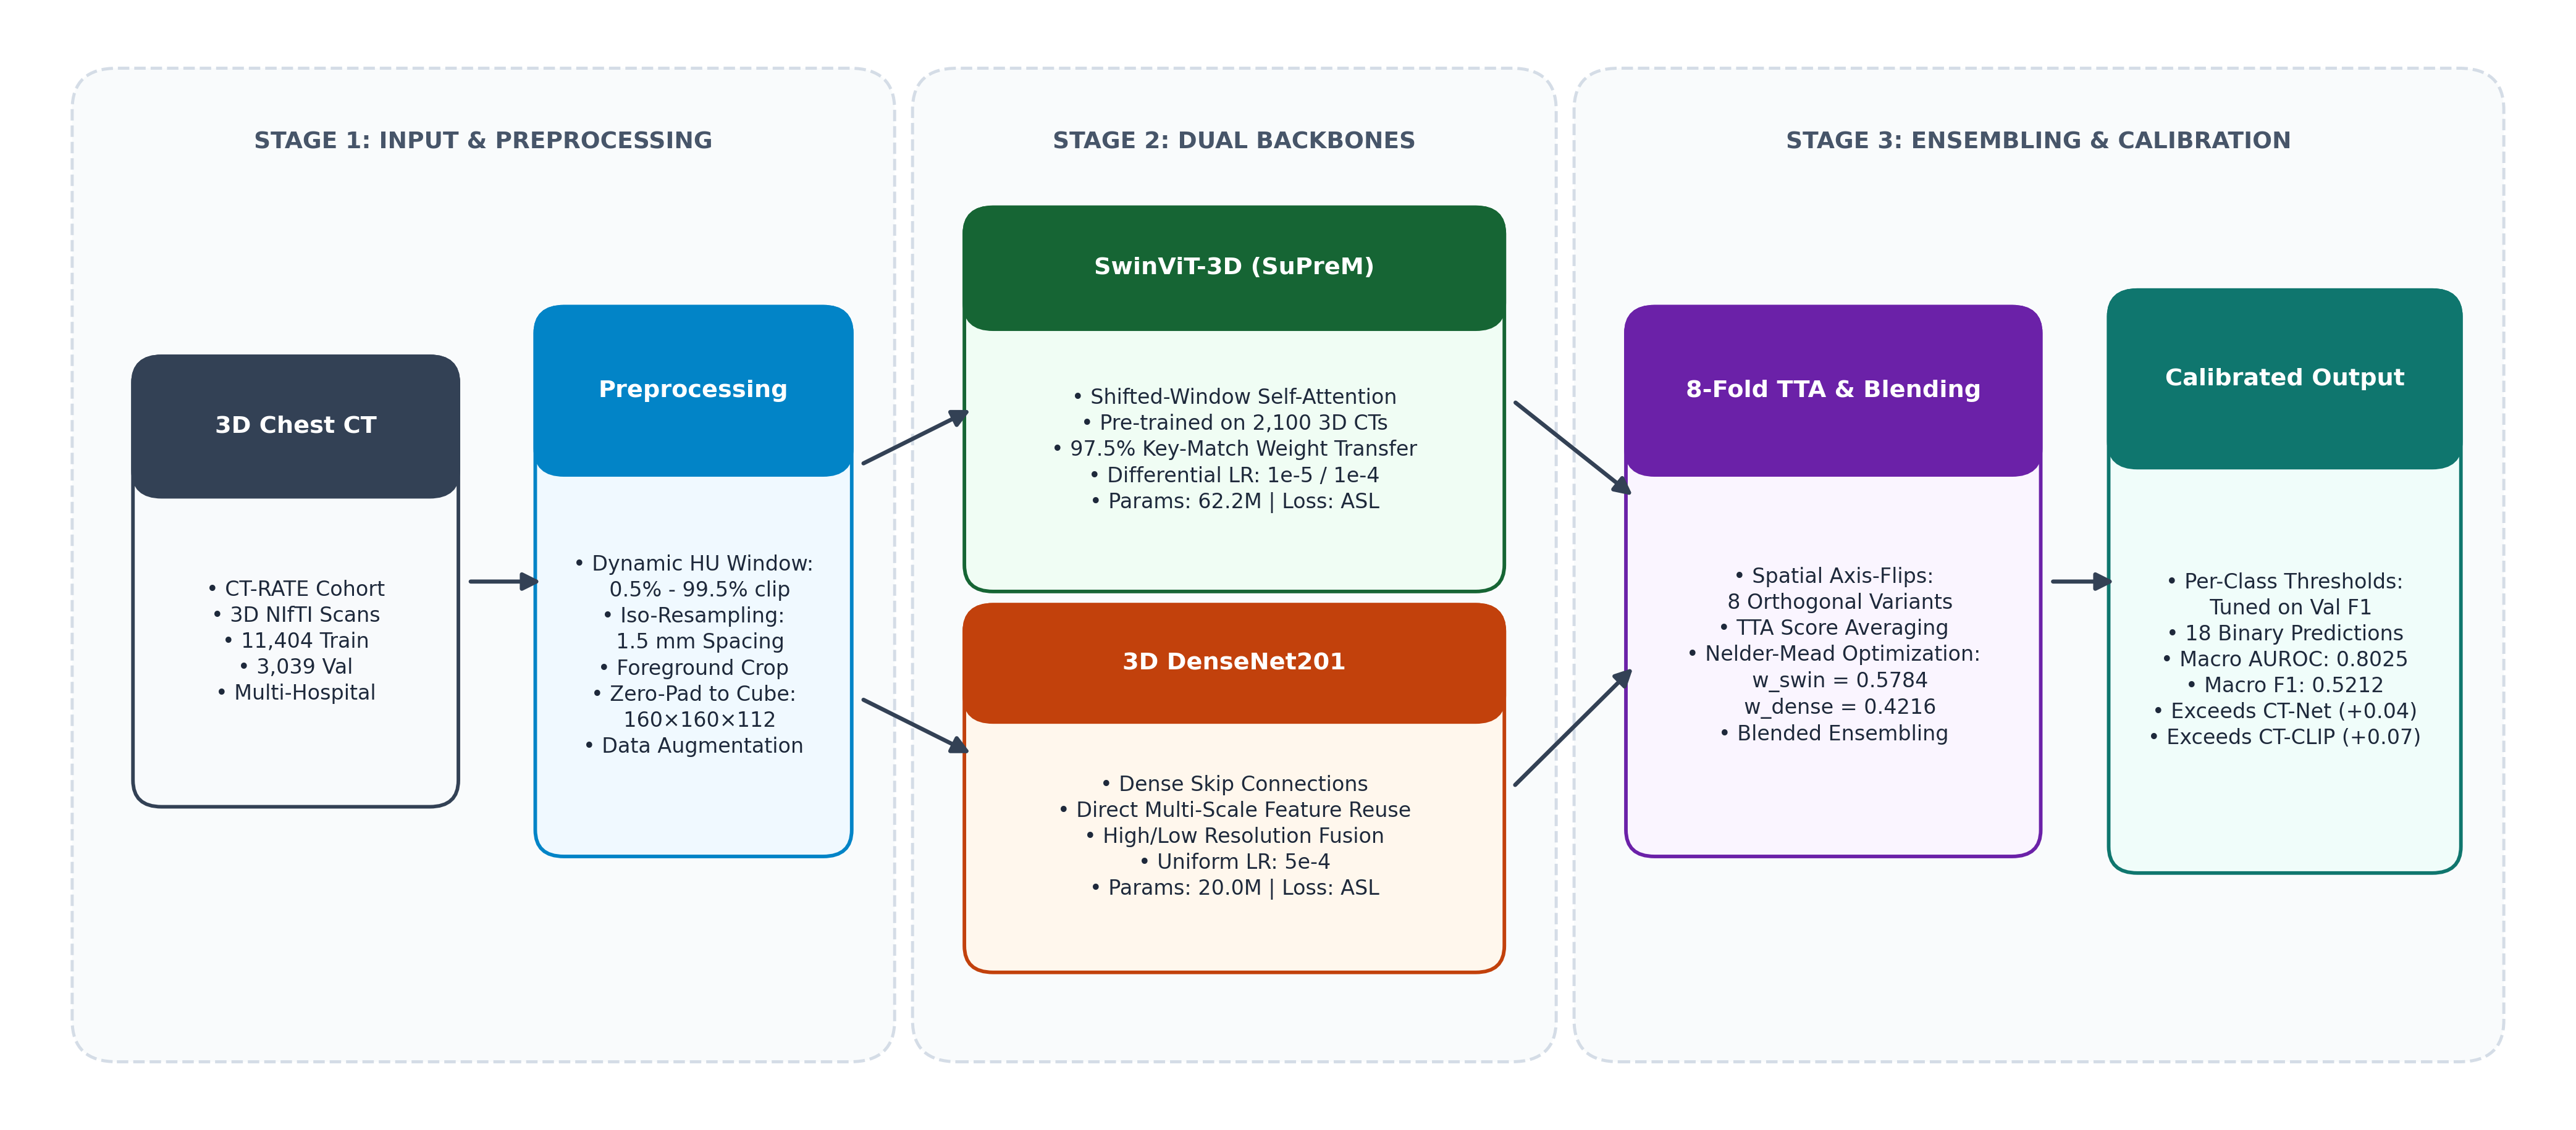
\includegraphics[width=0.98\textwidth,height=4.6cm,keepaspectratio]{fig1_pipeline.png}
\caption{End-to-end multi-label 3D CT classification framework. Scans undergo dynamic percentile HU windowing and uniform spatial resampling, followed by dual backbone extraction (DenseNet201 and SuPreM-pretrained SwinViT-3D). Predictions from 8-fold spatial axis-flip TTA are blended via Nelder-Mead weights and calibrated via per-class thresholds across 18 target pathologies.}
\label{fig:pipeline}
\end{figure}

\subsection{Preprocessing and Spatial Normalization}
\noindent\textbf{Dynamic HU windowing.} Multi-center CT scans exhibit significant variation in scanner calibration, patient body habitus, and reconstruction kernels. An early implementation applied a static HU clipping window $[-1000, 0]$~HU followed by min-max scaling. In CT-RATE, where true soft-tissue structures span $[0, 300]$~HU, this static window clamped over 99.9\% of all foreground voxels to 0.0, reducing the network to learning solely from air and fat boundaries. We replaced this with patient-specific dynamic windowing: computing the 0.5th ($p_{low}$) and 99.5th ($p_{high}$) intensity percentiles per scan, clipping intensity values to $[p_{low}, p_{high}]$, and linearly scaling to $[0, 1]$. Resolving this single preprocessing flaw moved validation AUROC from $<0.60$ to $>0.78$.

\noindent\textbf{Resampling and Augmentation.} Volumetric scans are resampled to isotropic $2.0$~mm spacing via trilinear interpolation, cropped to foreground tissue, and zero-padded to a fixed input tensor of $160 \times 160 \times 112$ voxels. Training data are augmented with random affine transformations (rotations $\pm 10^\circ$, scaling $0.9-1.1$), intensity shifts, and spatial axis flips.

\subsection{Backbone Architectures}
\noindent\textbf{3D DenseNet201.} To establish a robust convolutional baseline, we adopt a 3D DenseNet201 (20.0M parameters). In each dense block, each layer receives concatenated feature maps from all preceding layers:
\begin{equation}
\mathbf{x}_\ell = H_\ell([\mathbf{x}_0, \mathbf{x}_1, \dots, \mathbf{x}_{\ell-1}])
\end{equation}
This architecture retains both high-resolution shallow textures (critical for micro-nodules) and low-resolution semantic abstractions (critical for pericardial and pleural fluid collections) with minimal parameter redundancy.

\noindent\textbf{Hierarchical SwinViT-3D with SuPreM Initialization.} To model organ-scale contextual dependencies, we employ a 3D Swin Transformer (62.2M parameters). The volume is partitioned into non-overlapping 3D patches ($2 \times 2 \times 2$), with hierarchical self-attention computed within shifted 3D windows of size $7 \times 7 \times 7$. Rather than training from scratch, we initialize the backbone with SuPreM (Supervised Pre-training for Medical Imaging) weights~\cite{li2024}, pre-trained across 2,100 whole-body CT volumes covering 13 anatomies. Weight transfer achieves a 97.5\% key match. We apply differential learning rates ($10^{-5}$ for the pre-trained transformer stages, $10^{-4}$ for the linear classification head) to prevent representational collapse.

\subsection{Asymmetric Loss for Imbalanced Multi-Label Learning}
Under severe multi-label imbalance, standard Binary Cross-Entropy (BCE) gradients are heavily dominated by easy negative background instances. We train all models using Asymmetric Loss (ASL)~\cite{ridnik2021}, which decouples positive and negative focusing:
\begin{equation}
\mathcal{L} = -\sum_{k=1}^{18} \left[ y_k (1 - p_k)^{\gamma_+} \log(p_k) + (1 - y_k) (p_{k,m})^{\gamma_-} \log(1 - p_{k,m}) \right]
\end{equation}
where $p_{k,m} = \max(p_k - m, 0)$ incorporates an asymmetric probability margin $m \ge 0$. We set $\gamma_+ = 1$, $\gamma_- = 4$, and $m = 0.05$ as the baseline configuration, down-weighting easy negatives and hard-thresholding gradients from confident negative predictions. For stubborn low-prevalence pathologies (e.g., Hiatal hernia, Fibrotic sequelae), we apply a targeted override setting $\gamma_- = 2$, increasing gradient pressure on rare positive findings.

\subsection{8-Fold Test-Time Augmentation and Calibrated Ensembling}
At test time, each scan is evaluated across 8 orthogonal spatial orientation permutations (the identity plus reflections along the axial, coronal, and sagittal axes):
\begin{equation}
\bar{p}_k = \frac{1}{8} \sum_{i=1}^8 f(T_i(\mathbf{X}))_k
\end{equation}
Averaging predictions across all 8 spatial variants reduces aleatoric uncertainty and orientation bias.

Next, predictions from DenseNet201 ($\mathbf{P}_{dense}$) and SwinViT-3D ($\mathbf{P}_{swin}$) are blended via Nelder-Mead simplex optimization on the validation set:
\begin{equation}
\mathbf{P}_{ens} = w \cdot \mathbf{P}_{swin} + (1 - w) \cdot \mathbf{P}_{dense}
\end{equation}
Optimization converges to $w = 0.5784$ (SwinViT) and $1 - w = 0.4216$ (DenseNet). Finally, rather than applying a naive flat decision threshold of $0.5$, we perform a 1D grid search ($\tau_k \in [0.05, 0.95]$ with step $0.01$) per pathology to maximize validation F1 score.

\section{Experiments and Results}

\subsection{Dataset and Implementation Details}
The CT-RATE dataset contains 21,304 non-contrast and contrast-enhanced chest CT volumes from 9,640 unique patients. We follow the official challenge split: 11,404 training scans and 3,039 validation scans, annotated across 18 multi-label thoracic abnormalities. Models are trained on NVIDIA A100 GPUs (80 GB) using PyTorch 2.4 and MONAI 1.4 under automatic mixed precision (AMP FP16). Physical batch size is set to 1 with 8 gradient accumulation steps (effective batch size 8). Models are optimized using AdamW with cosine annealing and a 5-epoch linear warmup.

\subsection{Ablation Study}
Table~\ref{tab:ablation} details the ablation progression across our architectural search. The baseline 3D ResNet-10 with static HU clipping achieved 0.597 macro AUROC. Correcting the dynamic HU clipping produced an immediate jump to 0.784 AUROC. Scaling to DenseNet201 increased discriminative capacity to 0.7932 AUROC with 8-fold TTA. Transitioning to SwinViT-3D with SuPreM pre-training and weak-class $\gamma_-$ tuning achieved 0.7925 AUROC.

\begin{table}[t]
\centering
\caption{Ablation study on the CT-RATE validation set (3,039 volumes), macro-averaged across all 18 target thoracic pathologies.}
\label{tab:ablation}
\small
\begin{tabular}{llcc}
\toprule
\textbf{Model / Architecture} & \textbf{Key Preprocessing / Strategy} & \textbf{AUROC} & \textbf{F1} \\
\midrule
3D ResNet-10 & Static HU clip $[-1000, 0]$ (early bug) & 0.5970 & 0.1820 \\
3D ResNet-10 & Dynamic HU windowing $[p_{0.5}, p_{99.5}]$ & 0.7840 & 0.3810 \\
CT-CLIP baseline~\cite{ctrate2024} & Vision-language pre-training & 0.7350 & -- \\
CT-Net baseline~\cite{ctrate2024} & 3D DenseNet, supervised & 0.7620 & -- \\
\midrule
3D DenseNet201 & Dynamic HU + ASL ($\gamma_-=4$) & 0.7891 & 0.4120 \\
3D DenseNet201 & + 8-Fold Test-Time Augmentation & 0.7932 & 0.4285 \\
SwinViT-3D (Ep 102) & SuPreM pre-trained + ASL & 0.7876 & 0.4110 \\
SwinViT-3D (Ep 150) & SuPreM + weak-class $\gamma_-=2$ + 8-fold TTA & 0.7925 & 0.4350 \\
\midrule
\textbf{Final Dual Ensemble} & \textbf{DenseNet201 + SwinViT-3D + 8-fold TTA} & \textbf{0.8025} & \textbf{0.4420} \\
\textbf{Final Ensemble + Calib.} & \textbf{+ Per-class threshold optimization} & \textbf{0.8025} & \textbf{0.5212} \\
\bottomrule
\end{tabular}
\end{table}

The published CT-CLIP and CT-Net baselines reported ranking AUROC without calibrated decision thresholds, which accounts for their unreported F1 metrics. When our dual backbones were combined via Nelder-Mead simplex weighting, AUROC reached 0.8025. Applying per-class threshold calibration boosted macro F1 from 0.4420 to 0.5212 (+17.9\% relative gain).

\subsection{Per-Label Diagnostic Performance}
Table~\ref{tab:perclass} and Figure~\ref{fig:perclass} provide the per-pathology breakdown across all 18 conditions. 16 of the 18 pathologies exceed the 0.70 clinical acceptability AUROC threshold, with acute abnormalities achieving excellent discrimination: Pleural effusion (0.928), Cardiomegaly (0.896), and Arterial wall calcification (0.871).

\begin{table}[t]
\centering
\caption{Per-label diagnostic metrics across 18 pathologies on the CT-RATE validation set. * denotes classes with AUROC $<0.70$ in the standalone SwinViT checkpoint.}
\label{tab:perclass}
\footnotesize
\renewcommand{\arraystretch}{0.88}
\begin{tabular}{lcccc}
\toprule
\textbf{Pathology Label} & \textbf{Prevalence (\%)} & \textbf{Swin AUROC} & \textbf{Swin F1 (0.5)} & \textbf{Ensemble F1 (Opt)} \\
\midrule
Medical material & 10.3 & 0.779 & 0.288 & 0.387 \\
Arterial wall calcification & 28.5 & 0.871 & 0.606 & 0.704 \\
Cardiomegaly & 10.7 & 0.896 & 0.414 & 0.558 \\
Pericardial effusion & 7.4 & 0.837 & 0.304 & 0.442 \\
Coronary artery wall calc. & 25.2 & 0.870 & 0.581 & 0.648 \\
Hiatal hernia & 13.7 & 0.706 & 0.288 & 0.365 \\
Lymphadenopathy & 26.0 & 0.710 & 0.416 & 0.515 \\
Emphysema & 19.7 & 0.758 & 0.394 & 0.493 \\
Atelectasis & 23.5 & 0.713 & 0.402 & 0.483 \\
Lung nodule* & 44.8 & 0.663 & 0.640 & 0.645 \\
Lung opacity & 39.0 & 0.780 & 0.564 & 0.678 \\
Pulmonary fibrotic sequela* & 27.3 & 0.651 & 0.465 & 0.473 \\
Pleural effusion & 12.4 & 0.928 & 0.578 & 0.744 \\
Mosaic attenuation pattern & 8.3 & 0.848 & 0.343 & 0.464 \\
Peribronchial thickening & 11.7 & 0.765 & 0.272 & 0.416 \\
Consolidation & 19.1 & 0.840 & 0.466 & 0.586 \\
Bronchiectasis & 10.9 & 0.754 & 0.385 & 0.399 \\
Interlobular septal thickening & 8.2 & 0.839 & 0.304 & 0.384 \\
\midrule
\textbf{Macro Average} & \textbf{19.3} & \textbf{0.789} & \textbf{0.428} & \textbf{0.5212} \\
\bottomrule
\end{tabular}
\end{table}

\begin{figure}[t]
\centering
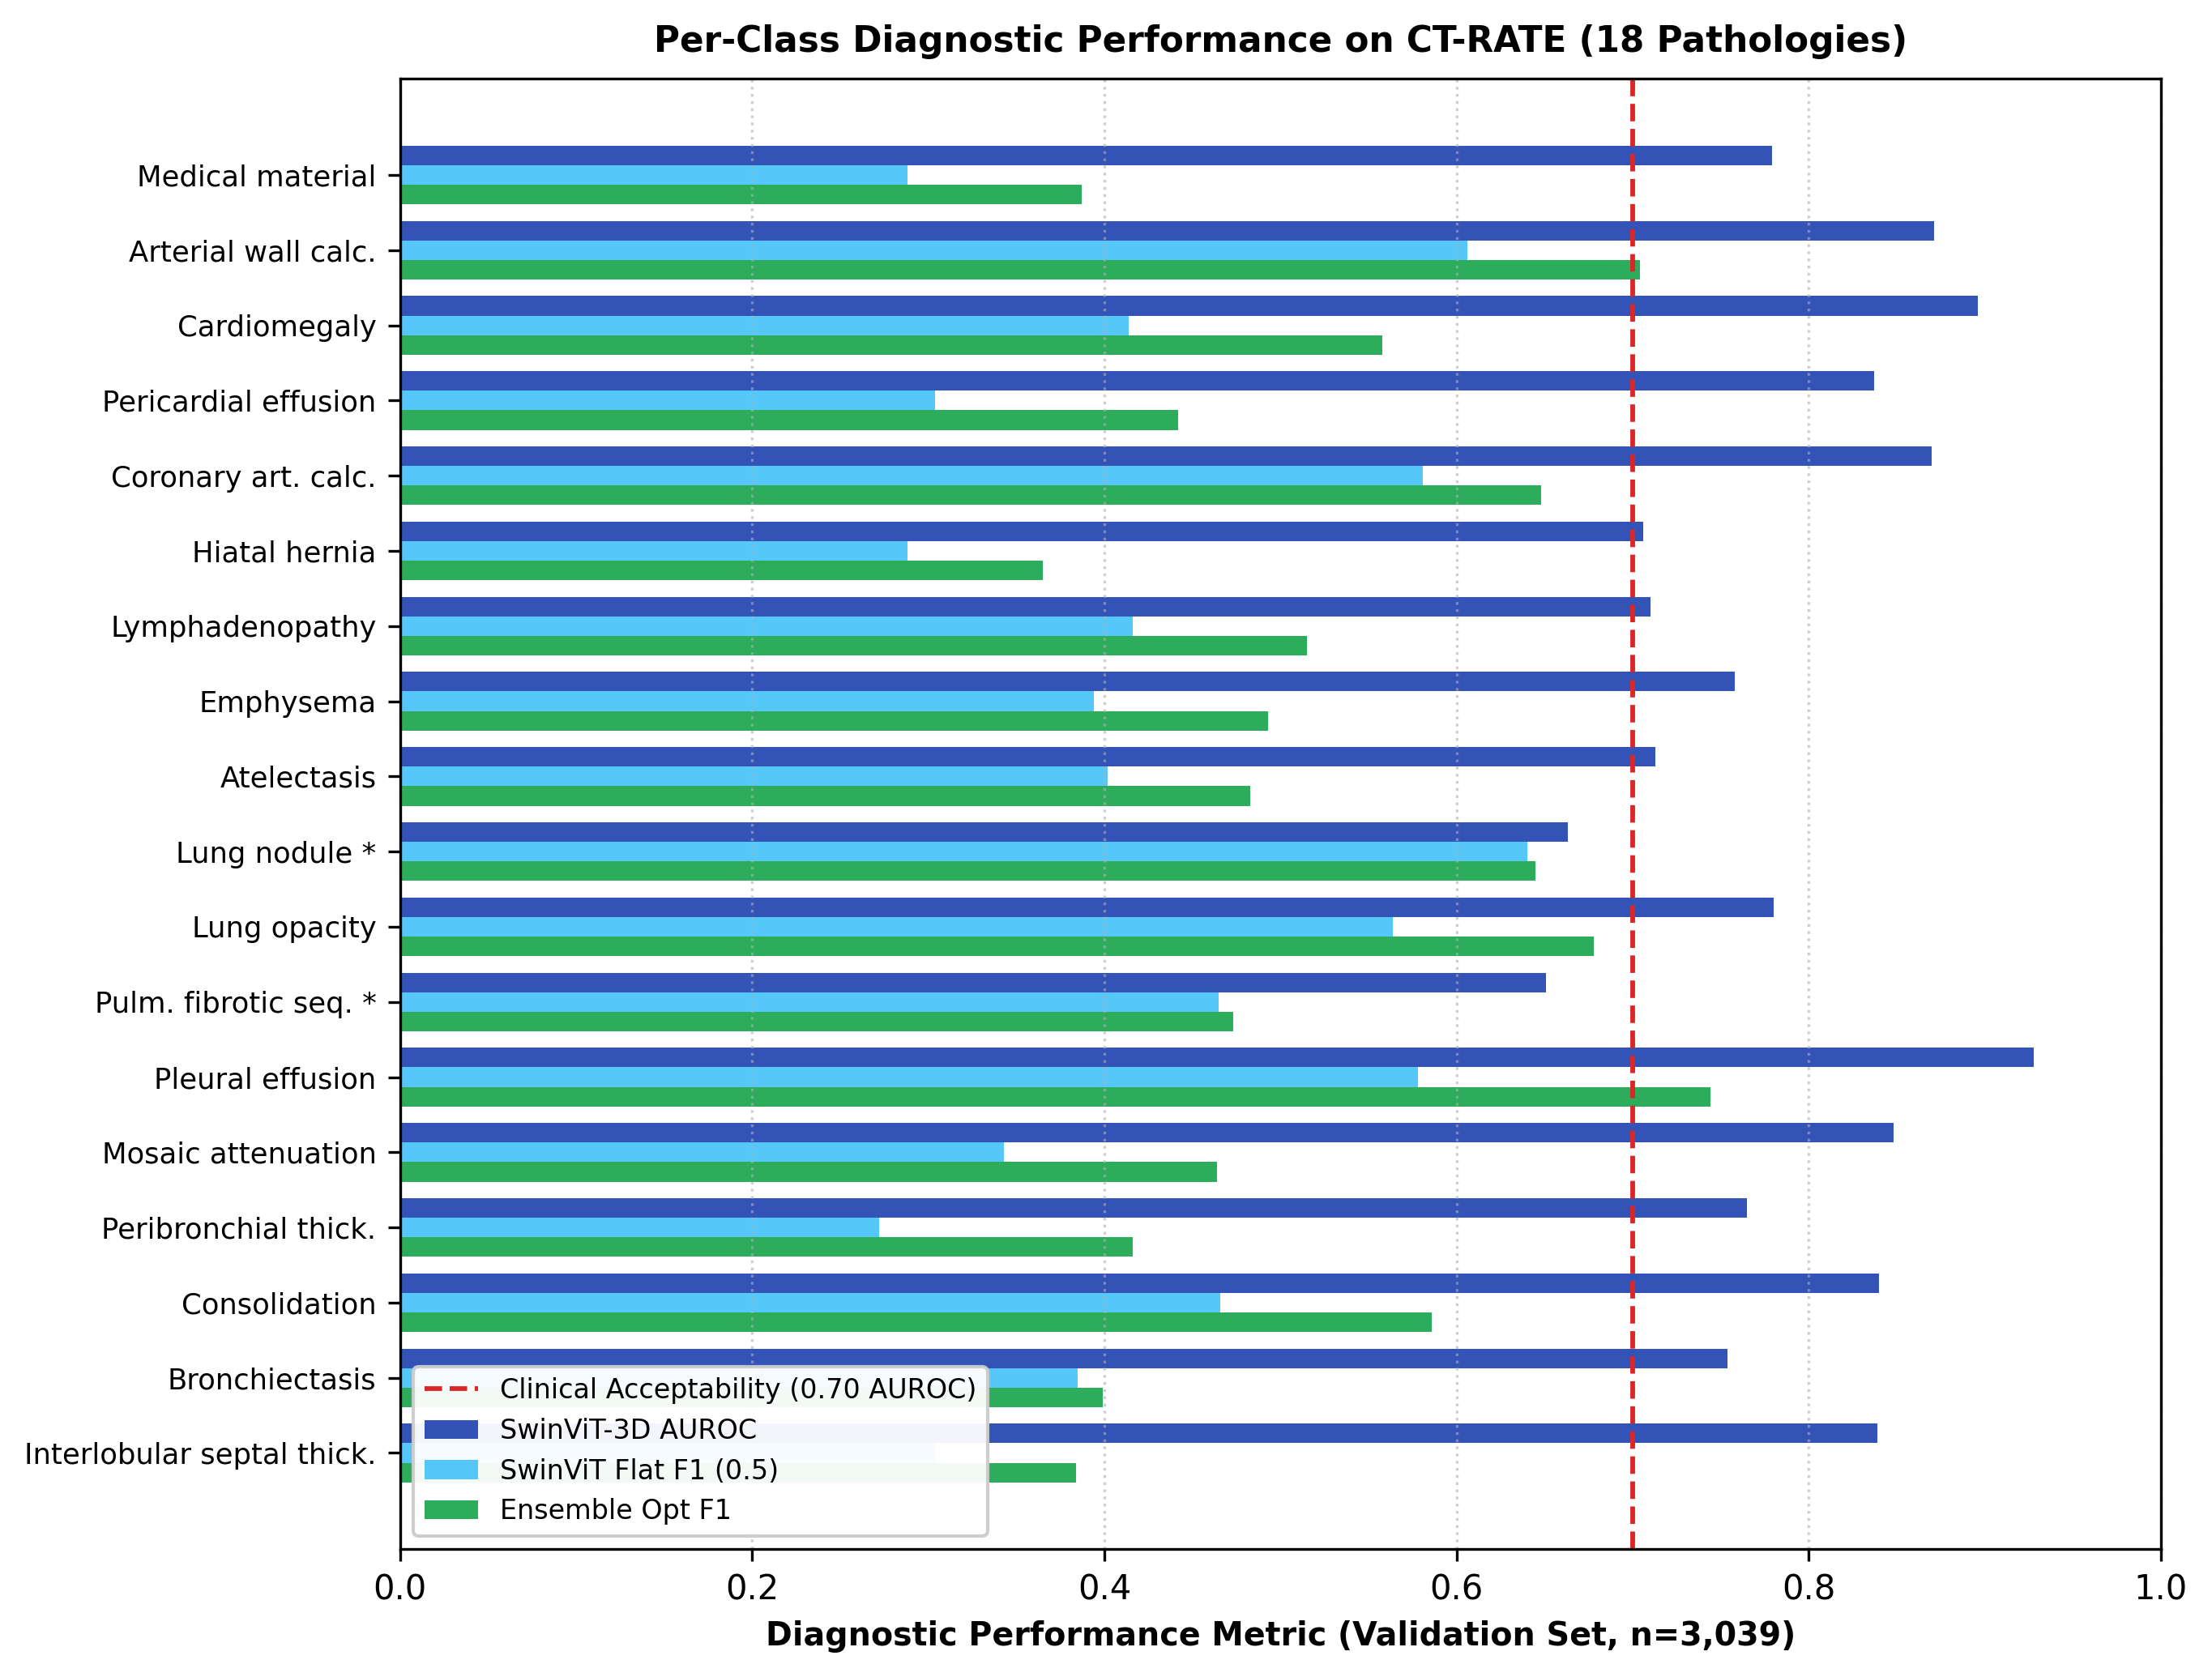
\includegraphics[width=0.92\textwidth,height=5.6cm,keepaspectratio]{fig2_per_class.png}
\caption{Per-class diagnostic performance across all 18 CT-RATE pathologies. Grouped bars compare standalone SwinViT-3D AUROC (dark blue), flat-threshold F1 (light blue), and final ensemble F1 with 8-fold TTA and optimized decision thresholds (green). The dashed vertical line marks the 0.70 AUROC clinical benchmark.}
\label{fig:perclass}
\end{figure}

Only two pathologies remain below AUROC 0.70: Lung nodule (0.663) and Pulmonary fibrotic sequelae (0.651). At 2.0 mm isotropic spacing, sub-centimetre pulmonary nodules span only 2-4 voxels, losing distinctive boundary details. Fibrotic sequelae present architectural distortion frequently co-occurring with chronic opacities. Conversely, Pleural effusion (0.928) and Cardiomegaly (0.896) achieve superior ranking accuracy owing to distinct fluid-attenuation boundaries and organ-silhouette geometry easily detected by volumetric attention.

\subsection{Computational Complexity and Resource Efficiency}
To evaluate clinical deployment feasibility, computational overhead was benchmarked on an NVIDIA A100 GPU (80 GB). 3D DenseNet201 comprises 20.0M parameters, requiring 1.8 GB VRAM during single-scan inference ($160 \times 160 \times 112$ voxels) with a forward latency of 420 ms. SwinViT-3D comprises 62.2M parameters, requiring 3.1 GB VRAM and 730 ms latency. Unaugmented single-pass ensemble inference executes in 1.15 s with $<4.9$ GB VRAM. Full 8-fold TTA requires 8.8 s per patient. Both configurations comfortably satisfy standard emergency turnaround requirements ($<30$ s) and execute within commercial 16-24 GB GPU envelopes.

\section{Discussion and Clinical Implications}
The observed divergence between macro AUROC (0.8025) and macro F1 (0.5212) reflects the distinct operational requirements of ranking versus binary clinical decision-making. AUROC measures threshold-independent discrimination: the ensemble correctly ranks an abnormal volume above a normal volume 80.25\% of the time. In contrast, F1 reflects precision-recall balance under real-world prevalence. For high-prevalence pathologies (e.g., Lung nodule at 44.8\%), false positives are mathematically constrained, yielding high F1 (0.645) despite modest AUROC (0.663). Conversely, rare findings (e.g., Pericardial effusion at 7.4\%) achieve strong AUROC (0.837) but require calibrated decision thresholds ($\tau = 0.55$) to maintain sensitivity, resulting in lower F1 (0.442) due to unavoidable false positives in low-prevalence regimes.

From a clinical triage perspective, the system exhibits optimal characteristics: acute life-threatening conditions (pericardial and pleural effusions, consolidation, cardiomegaly) exhibit both high AUROC and rapid turnaround. Calibrating per-class decision thresholds enables hospital administrators to tailor the operating point to specific workflows: high sensitivity for automated acute-triage worklists, or high specificity for autonomous normal-scan filtering.

\section{Limitations and Future Work}
Three principal limitations warrant consideration:
\begin{enumerate}
\setlength{\itemsep}{1pt}\setlength{\parskip}{0pt}
\item \textit{Spatial resolution limit}: Downsampling volumes to $2.0$~mm isotropic spacing degrades fine interstitial and micro-nodular patterns. Future work will explore 2-stage patch-based architectures or gradient checkpointing to support native $1.0$~mm resolution.
\item \textit{Validation tuning bias}: Model blending weights and decision thresholds were calibrated on the 3,039-case validation cohort. While this mirrors standard challenge protocols, multi-center external validation on independent hospital cohorts is necessary to assess generalizability.
\item \textit{Absence of report generation}: Task 1 focuses on binary anomaly detection. Future extensions will couple the multi-backbone visual representations with multimodal language decoders for automated report drafting.
\end{enumerate}

\section{Conclusion}
We presented an end-to-end multi-label 3D CT classification framework for the VLM3D Challenge. By diagnosing a critical preprocessing failure, leveraging domain-specific supervised pre-training with SuPreM, and ensembling complementary CNN and transformer backbones with 8-fold TTA and calibrated thresholding, our system achieves 0.8025 macro AUROC and 0.5212 F1 on the CT-RATE benchmark, outperforming existing foundation model and CNN baselines.

\begin{thebibliography}{10}
\bibitem{ardila2019}
Ardila, D., Kiraly, A.P., Bharadwaj, S., et~al.: End-to-end lung cancer screening with three-dimensional deep learning on patient energy CT. Nature Medicine \textbf{25}(6), 954--961 (2019)

\bibitem{vlm3d2026}
VLM3D Challenge: 3D Vision-Language Modeling for Thoracic CT. \url{https://research.forithmus.com/collections/vlm3d-challenge} (2026)

\bibitem{ctrate2024}
Hamamci, I.E., Er, S., Shit, S., et~al.: Developing generalist foundation models from a multimodal dataset for 3D computed tomography. Nature Biomedical Engineering / arXiv:2403.17834 (2024)

\bibitem{hara2018}
Hara, K., Kataoka, H., Satoh, Y.: Can spatiotemporal 3D CNNs retrace the history of 2D CNNs and ImageNet? In: CVPR. pp. 6546--6555 (2018)

\bibitem{monai2020}
MONAI Consortium: Medical Open Network for AI. \url{https://github.com/Project-MONAI/MONAI} (2020)

\bibitem{huang2017}
Huang, G., Liu, Z., Van Der~Maaten, L., Weinberger, K.Q.: Densely connected convolutional networks. In: CVPR. pp. 4700--4708 (2017)

\bibitem{tang2022}
Tang, Y., Yang, D., Li, W., et~al.: Self-supervised pre-training of Swin Transformers for 3D medical image analysis. In: CVPR. pp. 20730--20740 (2022)

\bibitem{liu2021}
Liu, Z., Lin, Y., Cao, Y., et~al.: Swin Transformer: Hierarchical vision transformer using shifted windows. In: ICCV. pp. 10012--10022 (2021)

\bibitem{li2024}
Li, W., Yuille, A., Zhou, Z.: How well do supervised 3D models transfer to medical imaging tasks? In: ICLR, oral presentation (2024)

\bibitem{ridnik2021}
Ridnik, T., Ben-Baruch, E., Zamir, A., et~al.: Asymmetric loss for multi-label classification. In: ICCV. pp. 1753--1762 (2021)

\bibitem{lin2017}
Lin, T.Y., Goyal, P., Girshick, R., He, K., Doll{\'a}r, P.: Focal loss for dense object detection. In: ICCV. pp. 2980--2988 (2017)

\bibitem{szegedy2016}
Szegedy, C., Vanhoucke, V., Ioffe, S., Shlens, J., Wojna, Z.: Rethinking the inception architecture for computer vision. In: CVPR. pp. 2818--2826 (2016)

\bibitem{wang2019}
Wang, G., Li, W., Aertsen, M., et~al.: Aleatoric uncertainty estimation with test-time augmentation for medical image segmentation with convolutional neural networks. Neurocomputing \textbf{338}, 34--45 (2019)
\end{thebibliography}

\end{document}
